\documentclass[10pt,english]{article}
\usepackage{babel,amsmath,amsfonts,amssymb,color,fancybox}
\usepackage{mathtools,microtype}
\usepackage{iftex}
\ifPDFTeX\usepackage[utf8]{inputenc}\fi
\usepackage[a4paper, inner=2.5cm, outer=2.5cm, top=2.0cm, bottom=2cm, bindingoffset=0cm]{geometry}
\usepackage{graphicx,booktabs,float,subcaption,placeins,adjustbox,siunitx,threeparttable}
\graphicspath{{../}}

%\usepackage{times}                  % stile delle sections

\newcommand{\reals}{\mathbf{R}}
\setlength{\parindent}{1.5em}
\setlength{\parskip}{1pt plus 0.5pt minus 0.5pt}
\raggedbottom
\setlength{\textfloatsep}{10pt plus 2pt minus 2pt}
\setlength{\floatsep}{8pt plus 2pt minus 2pt}
\setlength{\intextsep}{8pt plus 2pt minus 2pt}
\captionsetup{skip=4pt}
\captionsetup[subfigure]{font=footnotesize,skip=2pt}
\renewcommand{\topfraction}{0.9}
\renewcommand{\bottomfraction}{0.8}
\renewcommand{\textfraction}{0.07}
\renewcommand{\floatpagefraction}{0.82}
\sisetup{
  detect-all,
  group-digits=false,
  output-decimal-marker={.},
  table-number-alignment=center
}
%
\title{Review of Research Paper number 25\\ \large Homomorphically encrypted gradient descent algorithms for quadratic programming}
\date{version: \today}%Meeting held on: April the 2nd}
\author{Xiangyu Luo, Hamza Tarmadi, L\'ery Monnerat}
\begin{document}

\maketitle
%\small

\section{Introduction}

\subsection{Summary of the paper}

The paper addresses privacy-preserving solution of unconstrained quadratic programs via fully homomorphic encryption. It adapts the course algorithms GD and AGD to an encrypted setting and argues that CKKS is the suitable scheme because it supports approximate real arithmetic. Its main technical contribution is a matrix-multiplication procedure with lower multiplicative depth than JKLS-like constructions, which increases the number of feasible encrypted steps. The main numerical conclusion is that, under a fixed depth budget, GD is preferable for well-conditioned problems, whereas AGD is preferable for ill-conditioned ones. Hence the paper does not improve plain-text convergence theory, but it changes the practical ranking between GD and Nesterov-type acceleration once homomorphic-encryption constraints are imposed.

\subsection{Problem formulation}

Following the lecture-note notation, the paper studies the unconstrained optimization problem
\[
\min_{x \in \reals^n} f(x),
\qquad
f(x)=\frac{1}{2}x^\top Qx + p^\top x,
\]
where $Q=Q^\top \succeq 0$ and $p \in \reals^n$. This is a special case of the smooth convex problems considered in Section 1.2.3 of the notes, with feasible set $X=\reals^n$, so no projection step is needed. If $Q \succ 0$, then $f$ is differentiable, strongly convex, and admits the unique minimizer $x^\star$ characterized by
\[
\nabla f(x^\star)=Qx^\star + p = 0,
\qquad
x^\star = -Q^{-1}p.
\]
The paper does not use this closed-form formula because matrix inversion is not naturally compatible with the arithmetic primitives efficiently supported by homomorphic encryption. Instead, it evaluates first-order iterations on encrypted data.

The gradient and Hessian of the objective are
\[
\nabla f(x)=Qx+p,
\qquad
\nabla^2 f(x)=Q.
\]
Hence, in the notation of the lecture notes, $f \in S^1_{m,L}(\reals^n)$ whenever $Q \succ 0$, with
\[
m:=\lambda_{\min}(Q), \qquad L:=\lambda_{\max}(Q), \qquad \kappa:=\frac{L}{m}.
\]
The underlying plain-text algorithms are therefore the course methods
\[
x^{t+1}=x^t-\alpha_{\mathrm{GD}}(Qx^t+p),
\qquad
\alpha_{\mathrm{GD}}=\frac{2}{m+L},
\]
for gradient descent, and
\[
\begin{aligned}
y^{t+1}&=x^t-\alpha_{\mathrm{AGD}}(Qx^t+p), \qquad \alpha_{\mathrm{AGD}}=\frac{1}{L},\\
x^{t+1}&=(1+\beta)y^{t+1}-\beta y^t, \qquad \beta=\frac{\sqrt{\kappa}-1}{\sqrt{\kappa}+1},
\end{aligned}
\]
for accelerated gradient descent. The homomorphic-encryption layer changes the computation of $Qx^t$, but not the optimization model itself.

A direct connection with the course notes is obtained from kernel ridge regression. The notes write the Nystrom-approximated kernel problem as
\[
F(\alpha)=\frac{\sigma^2}{2}\alpha^\top K_{mm}\alpha+\frac{1}{2}\|y-K_{nm}\alpha\|_2^2+\frac{\nu}{2}\|\alpha\|_2^2.
\]
Expanding the square gives
\[
\frac{1}{2}\|y-K_{nm}\alpha\|_2^2
=
\frac{1}{2}\alpha^\top K_{nm}^\top K_{nm}\alpha
-y^\top K_{nm}\alpha
+\frac{1}{2}y^\top y,
\]
Discarding the constant term $\frac{1}{2}y^\top y$, one recovers the paper's quadratic program with
\[
Q=\sigma^2K_{mm}+K_{nm}^\top K_{nm}+\nu I,
\qquad
p=-K_{nm}^\top y.
\]
This reduction shows that the paper fits naturally into a concrete kernel example already present in the course material.

\subsection{Assumptions}

The assumptions of the paper can be divided into optimization assumptions and homomorphic-encryption assumptions.

\textit{Optimization assumptions.} The paper starts from a quadratic objective with symmetric positive semidefinite matrix,
\[
Q=Q^\top, \qquad Q \succeq 0.
\]
This is sufficient for the paper's gradient-descent convergence proposition. However, the comparison between GD and AGD, and the explicit use of the condition number $\kappa$, require the stronger hypothesis
\[
Q \succ 0.
\]
Under this condition, the objective is $m$-strongly convex and $L$-smooth, with $m=\lambda_{\min}(Q)>0$ and $L=\lambda_{\max}(Q)$. The user is also assumed to know these spectral bounds in plain text, since the step sizes of GD and AGD depend on them.

\textit{Homomorphic-encryption assumptions.} The paper argues that CKKS is the only suitable scheme among BFV, BGV, and CKKS, because gradient methods require non-integer step sizes. In the lecture-note notation, GD convergence needs $0<\alpha<2/L$; an integer-only arithmetic would make this condition unrealistically restrictive. A second assumption is that encrypted comparisons are not readily available, so classical stopping tests based on iterate differences or optimality gaps cannot be used directly. The number of iterations must therefore be fixed in advance. A third assumption is the existence of a finite multiplicative-depth budget, since ciphertext noise grows under multiplication. In the numerical section of the paper and of the present reproduction, the relevant budget is $18$.

\textit{Scope assumptions.} The paper treats only unconstrained QPs. Equality constraints are discussed only as future extensions, while inequality constraints remain difficult because they would require comparisons or projections inside the encrypted computation. For the reproduction considered here, one additional assumption is important: the implementation uses a \emph{simulated} CKKS backend rather than a full Microsoft SEAL pipeline. Therefore the optimization logic follows the paper faithfully, but the numerical section should be read as a paper-style reproduction and extension, not as a direct real-CKKS benchmark.

\section{Results: Theory and Practice}

\subsection{Theory}

The main formal result of the paper is Proposition 3.1, which is the lecture-note contraction theorem specialized to a quadratic objective. Let $x^\star$ denote the minimizer. Since $Qx^\star+p=0$, one GD step satisfies
\[
\begin{aligned}
x^{t+1}-x^\star
&=x^t-\alpha(Qx^t+p)-x^\star, \\
&=x^t-x^\star-\alpha(Qx^t-Qx^\star), \\
&=(I-\alpha Q)(x^t-x^\star).
\end{aligned}
\]
Because $Q$ is symmetric, the eigenvalues of $I-\alpha Q$ are $1-\alpha\lambda_i(Q)$, hence
\[
\|x^{t+1}-x^\star\|_2
\le
\rho(\alpha)\|x^t-x^\star\|_2,
\qquad
\rho(\alpha):=\max_i |1-\alpha\lambda_i(Q)|,
\]
Therefore, if $0<\alpha<2/L$, then $\rho(\alpha)<1$ and
\[
\|x^t-x^\star\|_2 \le \rho(\alpha)^t \|x^0-x^\star\|_2.
\]
This is exactly the linear convergence behavior proved in Theorem 1.1 of the notes. For the specific choice $\alpha_{\mathrm{GD}}=2/(m+L)$ one obtains the standard contraction factor $\rho_{\mathrm{GD}}=(\kappa-1)/(\kappa+1)$.

For AGD, the paper uses the usual strongly-convex parameters $\alpha_{\mathrm{AGD}}=1/L$ and $\beta=(\sqrt{\kappa}-1)/(\sqrt{\kappa}+1)$, so the asymptotic rate depends on $\sqrt{\kappa}$ rather than $\kappa$. In plain-text optimization this makes AGD preferable, especially when the conditioning is poor. The new contribution of the paper is to show that this ranking must be reconsidered once multiplicative depth becomes the scarce resource. The proposed matrix multiplication reduces the depth of one encrypted matrix product from $3$ for JKLS to $2$, and independent consistency checks confirm the resulting iteration caps under depth budget $18$.

\begin{table}[H]
\centering
\small
\begin{threeparttable}
\caption{Three-line comparison of encrypted matrix-multiplication cost models under depth budget $18$.}
\label{tab:mmult-costs}
\begin{tabular}{lccccc}
\toprule
Method & Ciphertexts & Complexity & Plain-cipher mult. & Depth & GD / AGD caps \\
\midrule
Halevi-Shoup & $d$ & $O(d^2)$ & 0 & 1 & -- \\
JKLS & 1 & $O(d)$ & 2 & 3 & 6 / 4 \\
Proposed & 1 & $O(d)$ & 1 & 2 & 9 / 6 \\
\bottomrule
\end{tabular}
\end{threeparttable}
\normalsize
\end{table}

Under the proposed matrix routine, one HE-GD step consumes depth $2$, while one HE-AGD step consumes depth $3$ because of the extra momentum update. Hence, under total depth budget $18$,
\[
N_{\mathrm{GD}}=\left\lfloor\frac{18}{2}\right\rfloor=9,
\qquad
N_{\mathrm{AGD}}=\left\lfloor\frac{18}{3}\right\rfloor=6.
\]
The interpretation is the main insight of the paper: under a fixed depth budget the relevant comparison is not between GD and AGD after the same number of iterations, but between the best iterate each method can reach before the circuit saturates. The numerical sweep of $100$ repetitions for each $(d,\kappa,\text{method})$ verifies exactly this threshold effect: for all tested dimensions $d \in \{2,4,8\}$, GD is preferred for $\kappa \in \{1.5,2,3,5\}$, while AGD is preferred for $\kappa \in \{10,20,50\}$. Thus the paper leaves the lecture-note convergence theory unchanged, but it changes the practical choice of first-order method by introducing multiplicative depth as an additional optimization resource. Figure~\ref{fig:numerics}(a) compares the analytical cost models, while Figure~\ref{fig:numerics}(b) displays the empirical crossover region.

\begin{figure}[tbp]
\centering
\begin{subfigure}[t]{0.48\linewidth}
\centering
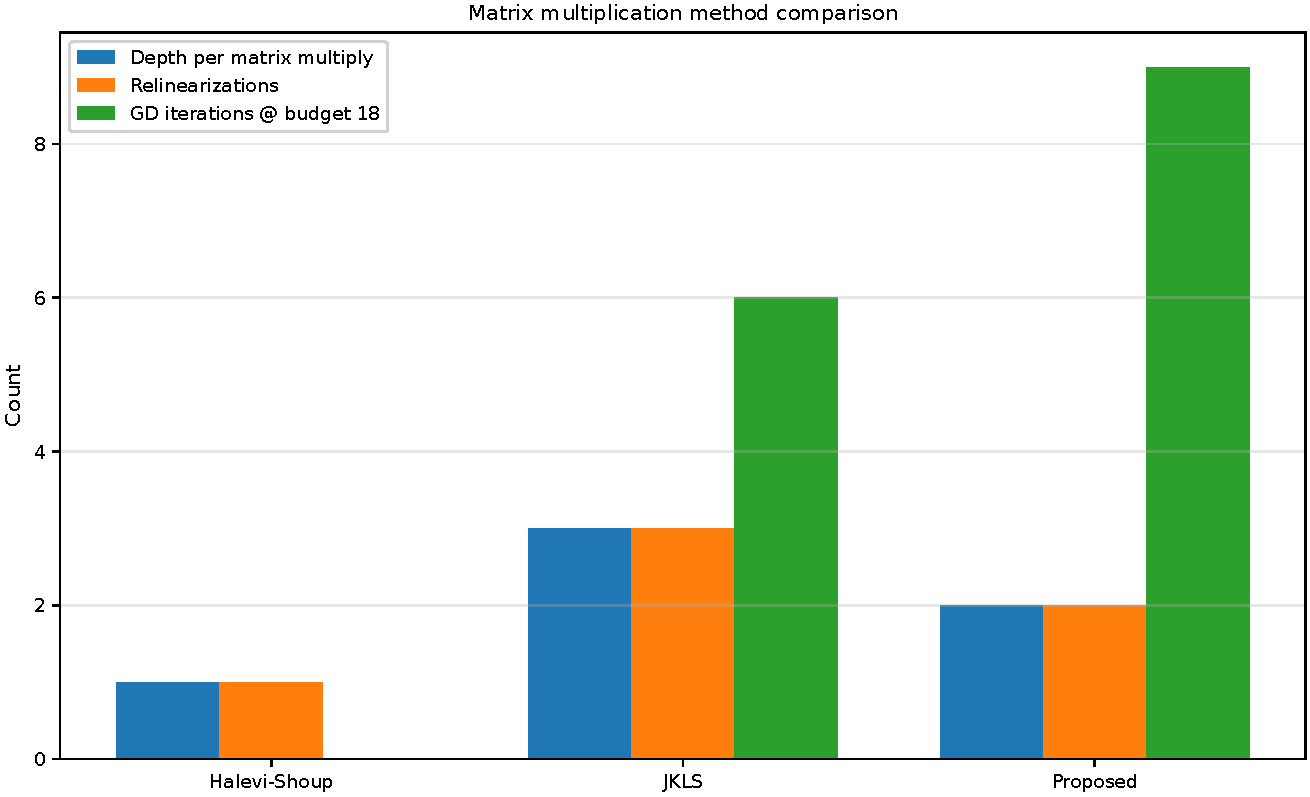
\includegraphics[width=\linewidth]{results/paper/paper_matrix_method_comparison.pdf}
\caption{Matrix-method cost comparison.}
\label{fig:panel-mmatrix}
\end{subfigure}
\hfill
\begin{subfigure}[t]{0.48\linewidth}
\centering
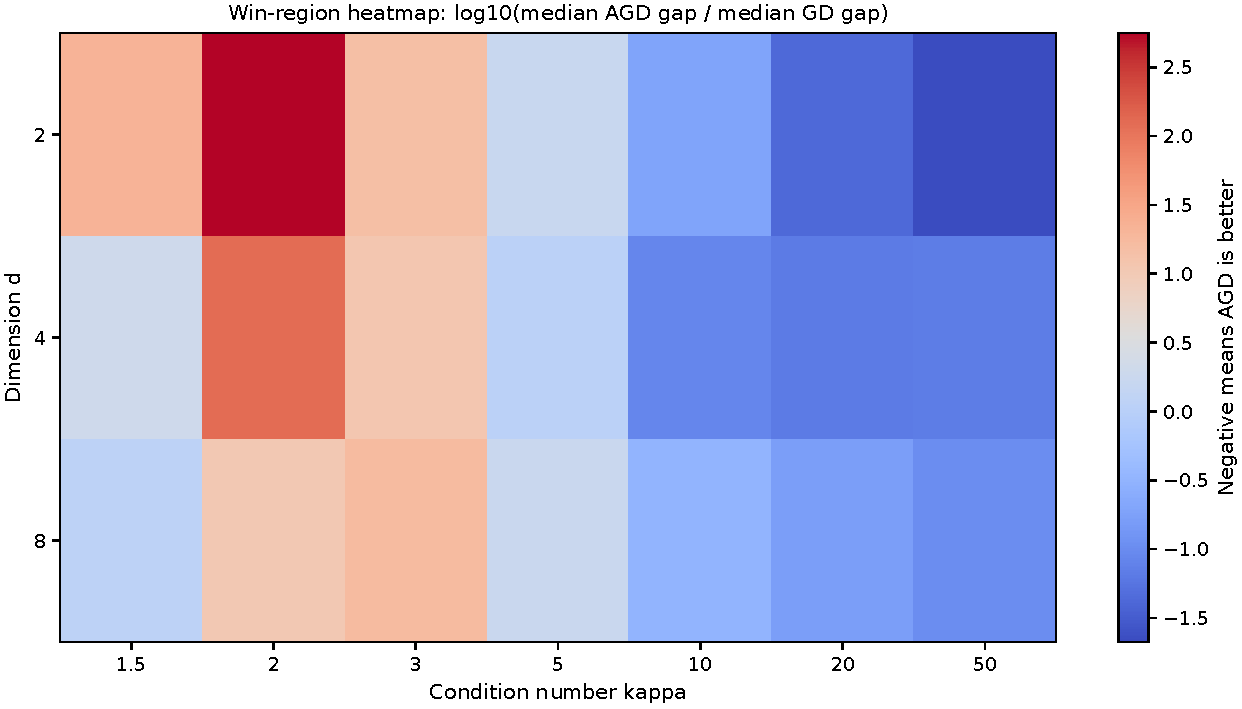
\includegraphics[width=\linewidth]{results/paper/paper_gd_vs_agd_win_region_heatmap.pdf}
\caption{Preferred encrypted method over $(d,\kappa)$.}
\label{fig:panel-heatmap}
\end{subfigure}

\vspace{0.3em}

\begin{subfigure}[t]{0.48\linewidth}
\centering
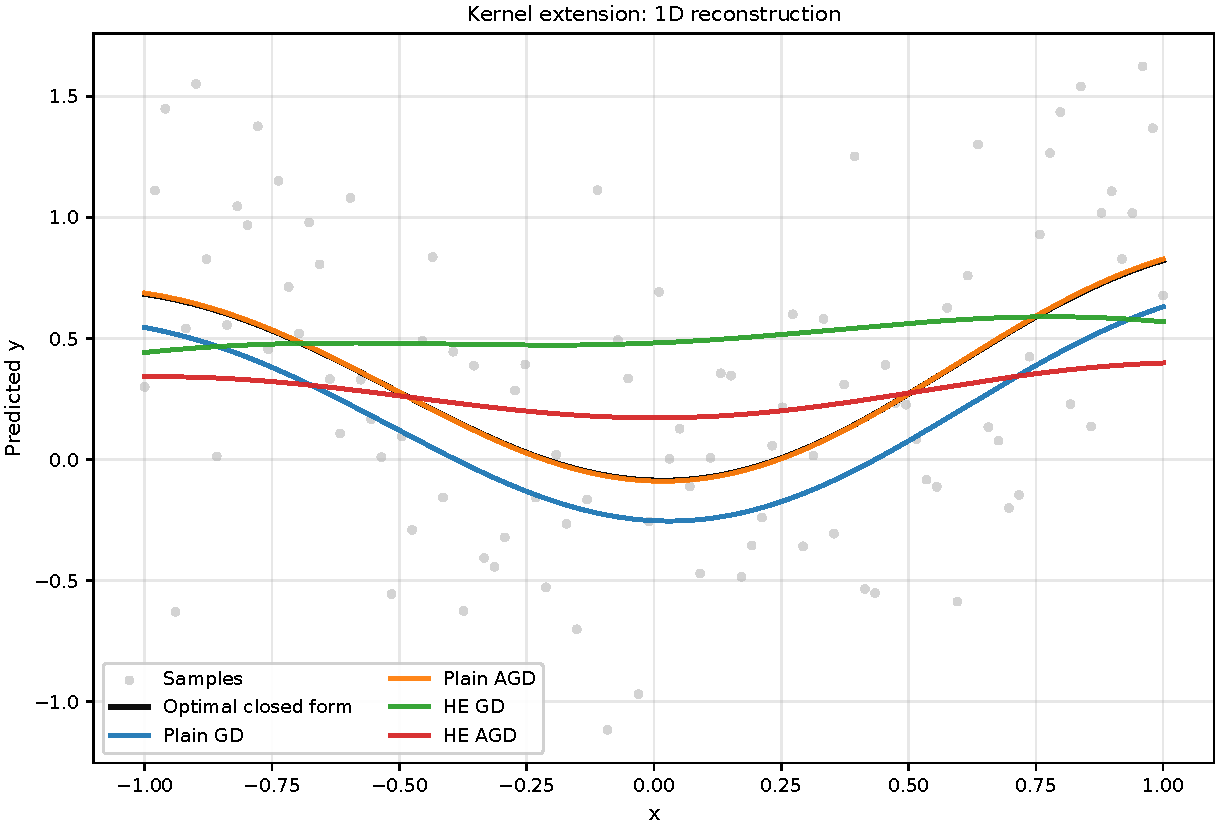
\includegraphics[width=\linewidth]{results/kernel/kernel_reconstruction.pdf}
\caption{One-dimensional kernel reconstruction.}
\label{fig:panel-reconstruction}
\end{subfigure}
\hfill
\begin{subfigure}[t]{0.48\linewidth}
\centering
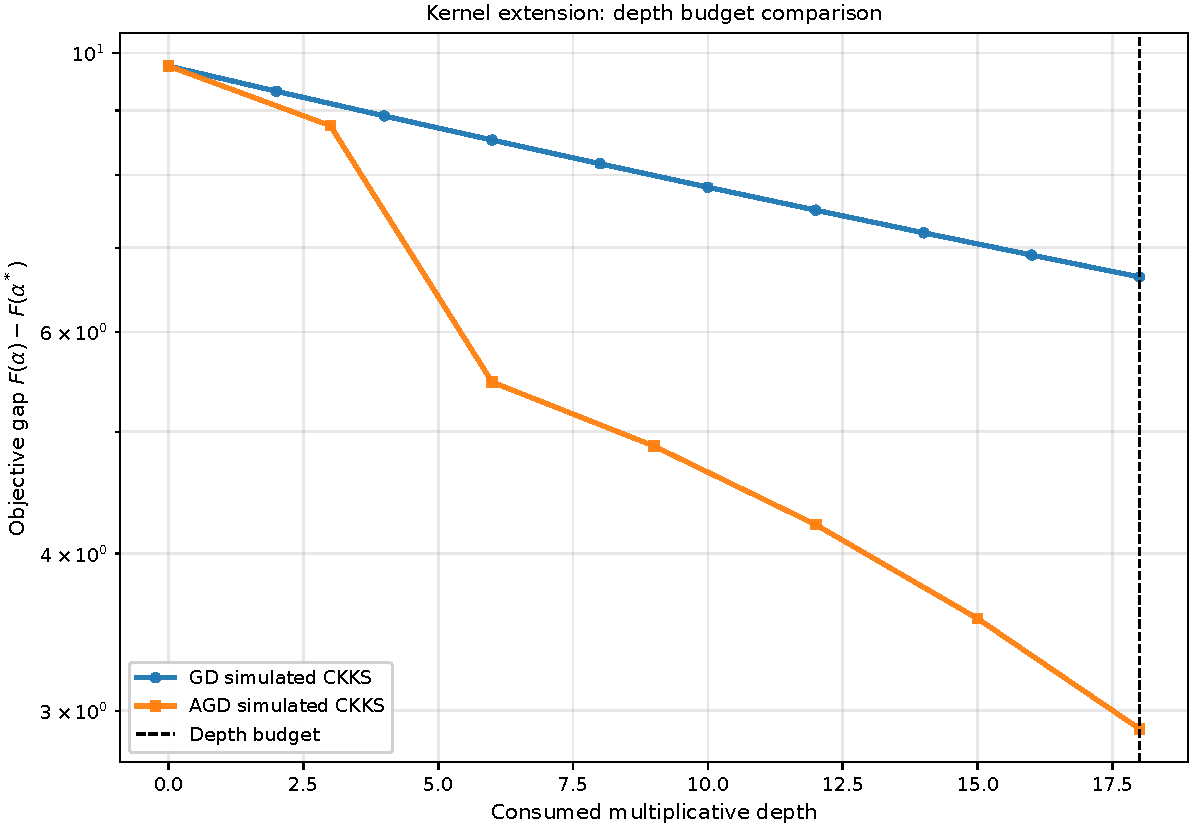
\includegraphics[width=\linewidth]{results/kernel/kernel_depth_budget_comparison.pdf}
\caption{Encrypted kernel performance versus consumed depth.}
\label{fig:panel-depth}
\end{subfigure}
\caption{Consolidated numerical evidence. Panels (a) and (b) summarize the theory-side comparison between encrypted GD and AGD under the multiplicative-depth model. Panels (c) and (d) report the corresponding kernel extension.}
\label{fig:numerics}
\end{figure}

\subsection{Practice}

The submitted code file is \texttt{he\_qp.py}, which is included in the accompanying code folder. This program was executed to generate the experiments reported in this subsection, and the same folder contains the corresponding figures, tables, and auxiliary outputs obtained from those runs. To test whether the paper's depth-limited GD/AGD tradeoff persists in the kernel setting of the course project, the Nystrom regression objective is rewritten in the coefficient vector $\alpha$ as $F(\alpha)=\frac{1}{2}\alpha^\top Q\alpha + p^\top \alpha$, with the same quadratic-program structure as in the paper. The numerical study then compares plain GD, plain AGD, simulated HE-GD, and simulated HE-AGD. For the kernel instance considered here, the resulting quadratic program has dimension $10$, condition number $\kappa \approx 387.83$, and parameters $\sigma = 0.5$ and $\nu = 1.0$, so the problem lies in the ill-conditioned regime where the theory predicts an advantage for AGD.

\begin{table}[H]
\centering
\small
\begin{threeparttable}
\caption{Kernel-extension results for the course baselines and their encrypted counterparts.}
\label{tab:kernel-results}
\begin{tabular}{
  l
  S[table-format=2.0]
  S[table-format=2.0]
  S[table-format=1.4]
  S[table-format=1.4]
}
\toprule
{Method} & {Iterations} & {Final depth} & {Final gap} & {Coeff. error} \\
\midrule
Plain GD & 80 & 80 & 1.5182 & 0.1390 \\
Plain AGD & 80 & 80 & \num{4.71e-4} & 0.0124 \\
HE-GD & 9 & 18 & 6.6354 & 1.0779 \\
HE-AGD & 6 & 18 & 2.9020 & 0.9672 \\
\bottomrule
\end{tabular}
\begin{tablenotes}[flushleft]
\footnotesize
\item The plain runs report the executed iteration count in the ``Final depth'' column; the encrypted runs report consumed multiplicative depth.
\end{tablenotes}
\end{threeparttable}
\normalsize
\end{table}

Since $Q\alpha^\star+p=0$ at the kernel optimum and $Q$ is symmetric, the identity $F(\alpha)-F(\alpha^\star)=\frac{1}{2}(\alpha-\alpha^\star)^\top Q(\alpha-\alpha^\star)$ shows that the final gap and the coefficient error in Table~\ref{tab:kernel-results} measure the same deviation in the $Q$-induced and Euclidean geometries, respectively. The practical conclusions are therefore clear. First, the plain-text baselines strongly favor AGD: after $80$ iterations the AGD gap is already below $10^{-3}$, whereas GD remains above $1$. Second, the encrypted methods are much less accurate because the depth budget of $18$ truncates the iterations at $9$ for HE-GD and $6$ for HE-AGD. Third, the ordering predicted by the theory is preserved: on this highly ill-conditioned kernel problem, HE-AGD still outperforms HE-GD. This is visible in Figure~\ref{fig:numerics}(c), where the HE-AGD reconstruction lies closer to the closed-form curve, and in Figure~\ref{fig:numerics}(d), where the AGD gap decreases more rapidly as multiplicative depth is consumed. The numerical study is thus consistent with the theoretical depth model, while remaining a simulated-CKKS reproduction rather than a hardware-level benchmark of deployed homomorphic-encryption software.

\section{Conclusion}

This paper shows how a familiar smooth strongly convex quadratic problem from the course changes once encrypted computation imposes a hard depth budget. The optimization model remains in $S^1_{m,L}$, so the lecture-note analysis of GD and AGD still applies, but the relevant performance criterion is no longer asymptotic rate at equal iteration count. Instead, one must compare the best accuracy achievable at equal multiplicative depth. In that regime, the paper does not introduce a new descent method; rather, it changes the practical ranking of existing first-order methods. The kernel experiment confirms that this message is not restricted to synthetic QPs, since the same GD/AGD crossover appears after rewriting kernel regression as a quadratic program. From the viewpoint of the course, the paper is therefore a useful example of how implementation constraints can modify algorithm selection without changing the underlying convex-optimization theory.

\end{document}
